%!TEX root=../main.tex

\section*{Аннотация}

DSLab - программный фреймворк для имитационного моделирования и тестирования распределенных систем.

В проекте используется дискретно-событийный подход описания моделей и приложений, где события обрабатываются в пользовательских функциях (callback-ах). В рамках проекта предстоит добавить возможность управлять событиями асинхронно.

\section*{Ключевые слова}

Распредленные системы, симуляция, асинхронность 


\newpage 

\section{Введение}

\begin{enumerate}
    \item Распределенная система -- система, выполняющая определенную задачу по обработке данных и компьютерных вычислений и использующая для этого несколько независимых машин (узлов), каждый из которых обладает своими ресурсами, памятью и запущенными процессами.
    \item Симуляция -- это процесс создания модели реальной системы или процесса, которая может быть использована для изучения и предсказания поведения системы в различных условиях.
    \item DSLab -- программный фреймворк для имитационного моделирования и тестирования распределенных систем.
    \item Асинхронное программирование -- это парадигма программирования, основанная на неблокирующем ожидании, которое позволяет программам переключаться на выполнение других задач в ожидании длительных операций.
    \item Callback -- это функция или код, который передается в качестве аргумента другой функции или метода, для выполнения в более поздний момент в ответ на событие или операцию.
    \item Логирование -- хронологическая запись операций, выполненных в системе. Логирование позволяет сохранять информацию о состоянии системы, которую можно использовать для ее исследования и отладки.
\end{enumerate}

\newpage

\section{Введение}

\subsection{Описание проекта DSLab}

В силу широты охвата областей применения фреймворка он организован в виде набора слабо связанных программных модулей, использование которых будет осуществляться через их API. Это даст возможность пользователям фреймворка (исследователям, разработчикам, преподавателям) гибким образом собирать из модулей решения под свои цели, например симуляторы для конкретных типов систем или постановок задач.

Входящие в состав фреймворка модули можно условно разделить на три типа:
\begin{enumerate}
    \item 
    Базовые, функциональность которых используется остальными модулями (например, 
    
    реализация дискретно-событийного моделирования)
    \item
    Универсальные, функциональность которых может быть использована в различных предметных областях (например, модели сети);
    \item
    Специализированные, которые заточены под определенную предметную область (например, библиотеки для моделирования облачных инфраструктур, исследования алгоритмов планирования заданий на кластерах или тестирования решений учебных заданий).
\end{enumerate}

Архитектуру DSLab можно схематично представить в виде трех слоев (Рис. \ref{dslab_arc}), включающих модули соответствующего типа. На рисунке также указаны текущие модули и зависимости между ними. Зависимости от dslab-core (от него зависят все имеющиеся универсальные и специализированные модули) не указаны, чтобы не загромождать рисунок. Таким образом, модули могут зависеть от модулей с нижних слоев, но не наоборот.

\begin{figure}[H]
    \centering
    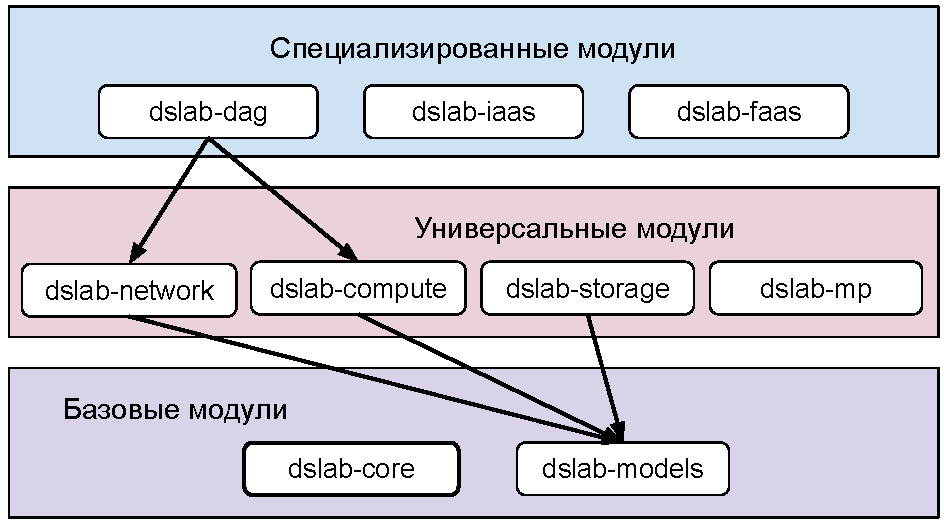
\includegraphics[width=0.7\linewidth]{images/dslab_arc.png}
    \caption{Архитектура DSLab}
    \label{dslab_arc}
\end{figure}

Описание архитектуры основано на документации проекта \cite{dslab-architecture}. Более подробно про проект можно прочитать в его описании \cite{dslab-description}, его требования \cite{dslab-requirements} и сравнение с аналогами \cite{dslab-analog-cmp}. Реализации модулей представлены в репозитории \cite{dslab-repo}.

Таким образом пользователь при разработке собственной симуляции может либо использовать уже готовые разработанные компоненты, либо реализовывать свои и произвольно их связывать. 


Основным процессом создания симуляции является создание событий и написание процессов реагирования на них. Каждое событие представляет из себя следующую структуру: 
\begin{enumerate}
    \item идентификатор события 
    \item идентификатор компонента, создавшего событие 
    \item идентификатор компонента, которому это событие предназначено доставить 
    \item внутреннее время, когда событие должно наступить
    \item произвольные данные события (<<полезная нагрузка>>)
\end{enumerate}

Таким образом в процессе симуляции разные компоненты генерируют события друг для друга и с помощью низкоуровневого модуля dslab-core обмениваются ими. Чтобы как-то реагировать на событие, каждый компонент реализует единственный обобщенный метод в который dslab-core передает нужное событие. При обработке события компоненты генерируют новые и таким образом цикл симуляции замыкается. 

Получается, что сейчас реагировать на пришедшие события можно только в одном месте -- в той самой функции-callback которую позовет dslab-core. В случае, когда событий немного -- это лаконично выглядит и этим удобно пользоваться. Но в более сложных алгоритмах с большим количеством различных событий, и, что важнее, цепочками событий, на которые нужно последовательно реагировать, подобная модель становится не самой удобной. С такой единой точной входа многие последовательные логичные действия оказываются фрагментированы (разбросаны по разным участкам кода). 

Хотелось бы иметь альтернативную возможность писать на языке программирования более понятный с первого взгляда алгоритм.

Как раз такой возможностью является написание асинхронного кода. Тогда различные сложные куски логики можно было бы выносить в отдельные функции, держать их вместе, просто исполнение бы прерывалось в ожидании какого-то события, чтобы продолжить.

\subsection{Цель и основные требования}
\begin{itemize}
    \item Реализовать асинхронное расширение для существующего ядра dslab-core или реализовать альтернативное асинхронное ядро 
    \item Добавить примеры использования нового функционала высокоуровневыми компонентами
    \item Написать подробную документацию нового API и покрыть реализацию тестами.
    \item Новое ядро должно быть реализовано эффективно: не должны возникать дополнительные (ассимтотически) накладные расходы по сравнению со стандартным ядром.
\end{itemize}

\subsection{Структура работы}

TODO 

\subsubsection{Значимость проекта DSLab}

Практически все современные информационные и вычислительные системы являются распределенными. Связано это с растущими объемами вычислений и обрабатываемых данных, требованиями к производительности, надежности и масштабируемости. Алгоритмическое обеспечение распределенных систем (например, алгоритмы управления ресурсами, планирования задач, балансировки нагрузки, членства в группе, консенсуса) является предметом активных исследований. В силу масштабов современных систем, сложности их реализации и недетерминированного характера, исследование алгоритмов и тестирование их реализаций в реальных системах существенно затруднено. Поэтому часто подобные исследования проводятся на аналитических и имитационных моделях, описывающих существенные для решаемой задачи аспекты поведения системы и проводимых вычислений. Использование моделей позволяет значительно удешевить эксперименты, сократить время их проведения и обеспечить воспроизводимость их результатов \cite{dslab-description}. 

\subsubsection{Преимущества асинхронного подхода}

Как уже было описано в мотивации постановки цели этой работы, главное преимущество асинхронной модели~--~удобство при написании сложных многоступенчатых алгоритмов.

Это повысит читаемость кода. Процесс принятия решения о сохранении файла в распределенном хранилище в такой парадигме мог бы выглядеть таким образом (псевдокод):

\begin{figure}[H]
\begin{lstlisting}[language=Python]
    async fn add_file_to_storage(some_file) {
        send_file_to_all_replicas(some_file);
        result = wait_for_confirmation_from_all().await;
        if result.has_quorum {
            send_commit_to_all_replicas();
            wait_for_commit_confirmation_from_quorum(result.nodes).await;
            send_ok_message_to_user();
        } else {
            send_reject_message_to_user();
        }
    }
\end{lstlisting}
\caption{Псевдокод асинхронного взаимодействия нод в симуляции}
\label{pseudocode}
\end{figure}

Посмотрев на функцию можно понять, что она делает, потому что логика последовательна и удобно разбита на подфункции. У нас есть возможность написать такой алгоритм на верхнем уровне, а не обрабатывать сообщения всех типов от всех реплик в единой точке входа.

\subsubsection{Возможные недостатки асинхронного подхода}

Программировать в парадигме асинхронного взаимодействия требует соответствующей подготовки пользователя. Не смотря на то, что в любой момент времени исполняется только одна функция, и проблем многопоточного программирования вида \texttt{data-race} не возникает, нужно постоянно держать в голове, что <<параллельно>> могут быть запущены другие процессы, которые могли поменять общую память в то время, когда функция была неактивна. 

\newpage 

\section{Существующие работы и решения}

Подобный подход уже был реализован в других симуляторах, например в SimGrid \cite{simgrid-example}. Главное отличие подхода DSLab от SimGrid -- наличие дискретно-событийного моделирования. В SimGrid компоненты общаются между собой асинхронно через MailBox-ы (аналог канала из языка Go). Также код из примера сложно назвать легко читаемым, потому что SimGrid -- низкоуровневый фреймворк.

Более близким к желаемой реализации является использование корутин языка Kotlin в проекте OpenDC~\cite{opendc-repo}. К сожалению, проект не содержит достаточно разнообразных примеров использования симуляции в асинхронном контексте, но простой пример запуска симуляции в асинхронном контексте~\cite{opendc-example} очень похож на ожидаемый опыт использования асинхронности в DSLab.


Опыт других проектов не очень хорошо подходит как опора для разработки нового решения из-за специфики языка Rust и внутренней архитектуры симулятора.


\section{Управление исполнением}

Чтобы дать возможность пользователю писать асинхронный код, нужно создать саму возможность обрабатывать события асинхронно. Для этого нужно написать свой executor задач в DSLab, который будет исходя из внутренней логики (наступление времени, когда событие нужно доставить получателю) понимать, когда и какую асинхронную задачу нужно разбудить, и дать ей продолжить исполнение. 

К счастью, язык Rust дает возможность пользователям самим управлять процессом рантайма: с помощью библиотеки futures \cite{rust-futures} такое поведение может быть реализовано (что на простом примере и описано в официальной документации \cite{async-book}).

В основе подхода асинхронного исполнения в языке Rust лежат stackless-корутины. Каждая асинхронная функция превращается в state-machine. На высоком уровне это объект с фукнциями-callback-ами, внутри которых нет асинхронного ожидания. Т.е. компилятор <<разрезает>> за нас эту функцию на части, которые нам нужно будет исполнить. Это ровно то, что сейчас разработчик, использующий DSLab делает самостоятельно. В существующей модели исполнения каждый компонент предоставляет ядру набор callback-ов на каждое событие, которые должен написать пользователь. Из-за этого код получается искусственно <<разрезан>> на части в местах ожидания событий. В асинхронном подходе мы пишем стандартную фукнцию, используя \texttt{.await} для ожидания, и компилятор разрезает эту функцию за нас. Наглядно можно продемонстрировать разницу на вот таком участке эквивалентного псевдокода: 

\begin{figure}[H]
    \centering
    \begin{subfigure}[b]{0.45\linewidth}
        \centering
        \begin{lstlisting}[language=Python]
fn on_first_action(&self) {
    // do 1
}
fn on_first_event(&self) {
    // do 2
}
fn on_second_event(&self) {
    // do 3
}
    \end{lstlisting}
        \caption{Синхронный код (разрезан на части разработчиком)}
        \label{sync-async-example:sync}
    \end{subfigure}
    \hfill
    \begin{subfigure}[b]{0.45\linewidth}
        \centering
        \begin{lstlisting}[language=Python]
async fn action(&self) {
    // do 1
    wait_for_first_event().await;
    // do 2 
    wait_for_second_event().await;
    // do 3
}
    \end{lstlisting}
        \caption{Асинхронный код (разрезан на части компилятором)}
        \label{sync-async-example:async}
    \end{subfigure}
\caption{Сравнение синхронного и асинхронного кода на языке Rust}
\label{sync-async-example}
\end{figure}

Как можно ожидать, ни один из этих примеров не исполняется сам. В случае синхронного примера (\ref{sync-async-example:sync}) очевидно, что у него нет <<единой точки запуска>>, т.е. каждую из трех функций-callback-ов должно позвать ядро исполнения симуляции (dslab-core). 

Для асинхронного примера (\ref{sync-async-example:async}) действует то же самое правило: на при наступлении соответствующего события нужно <<разбудить>> эту функцию и дойти до следующего места ожидания. Именно такую возможность и нужно поддержать в dslab-core. 

Главный компонент исполнителя задач -- логика, по которой нужно ставить на исполнение ту или иную задачу в dslab-core уже реализована. Это и есть основа всей дискретно-событийной симуляции. Остается только добавить возможность <<возобновлять>> исполнение асинхронной функции как раз в том месте, где сейчас вызывается заранее зарегистрированный пользовательский callback.


\section{Дизайн и структура ядра DSLab}

\subsection{Событие} \label{Event}
Основа дискретно-событийного моделирования -- события. В фреймворке DSLab они представленны структурой \underline{\texttt{Event}} со следующими полями: 
\begin{itemize}
    \item \texttt{id: EventId} -- уникальный идентификатор события во всей симуляции
    \item \texttt{time: f64} -- время наступления события 
    \item \texttt{src: Id} -- идентификатор компонента симуляции, создавший это событие 
    \item \texttt{dest: Id} -- идентификатор компонента симуляции, которому это событие предназначается
    \item \label{Event:payload} \texttt{data: Box<dyn EventData>} -- произвольная <<полезная нагрузка>> события, которая может иметь любой тип и определяется пользователем. 
\end{itemize}

\subsection{Обработчик событий} \label{EventHandler}

Обрабатывать события симуляции в DSLab может любой класс, реализующий интерфейс \underline{\texttt{EventHandler}}. Этот интерфейс содержит единственную функцию: 
\begin{center}
\texttt{fn on(\&mut self, event: Event)}
\label{fnon}
\end{center}

Именно эта функция вызывается как callback для обработки полученного события.

\subsection{Основные классы симуляции}
Модуль dslab-core состоит из нескольких основных классов, логически разделенных друг от друга:
\begin{itemize}
    \item \texttt{Simulation} -- основной класс, отвечающий за симуляцию. С него начинается создание любой симуляции. Он же предоставляет API для контроля за событиями. Основные методы:
    \begin{itemize}
        \item \label{Simulation::step} \texttt{Simulation::step() -> bool} -- сделать один <<шаг>> симуляции. Это значит взять из очереди событие с наименьшим временем наступления и вызвать обработчик у компонента, которому это событие предназначается. Возвращает \texttt{true} если все перечисленные действия успешно завершились. 
        \item \texttt{Simulation::time() -> f64} -- вернуть текущее время симуляции (вещественное число). Оно совпадает с временем последнего обработанного события. 
        \item \label{Simulation::createcontext} \texttt{Simulation::create\_context(name: \&str) -> SimulationContext} -- Создать контекст для компонента с именем \texttt{name} симуляции, с помощью которого тот будет отправлять события.
    
        \item \texttt{Simulation::add\_handler(name: \&str, handler: dyn EventHandler)} -- Добавить обработчик событий для компонента с именем \texttt{name}.
        Этот метод принимает любой класс, реализующий публичный интерфейс \hyperref[EventHandler]{EventHandler}. Когда компоненту \texttt{name} нужно будет доставить какое-либо событие (в рамках исполнения метода \hyperref[Simulation::step]{Simulation::step()}), именно эта функция будет вызвана для обработки события.
        \item Набор методов для генерации псевдослучайных последовательностей. Опустим эти детали, поскольку эта часть не очень важна в данной работе.
    \end{itemize}
    \item \texttt{SimulationState} -- класс состояния симуляции. Является полем класса \texttt{Simulation} и хранит в себе всю информацию о симуляции: очереди событий и отмененные события.
    \item \texttt{SimulationContext} -- контекст одного компонента симуляции. Является продуктом вызова функции \hyperref[Simulation::createcontext]{Simulation::create\_context}. В предполагаемом дизайне системы является полем класса, отвечающем за функционал отдельного компонента симуляции. Основные методы API для взаимодействия с симуляцией:
    \begin{itemize}
        \item \texttt{SimulationContext::emit<T>(data: T, dest: Id, delay: f64) -> EventId} -- добавить в симуляцию событие. Принимает данные произвольного типа T и создает \hyperref[Event]{событие} с этими данными, которое должно быть доставленно компоненту симуляции с идентификатором \texttt{dest} через время \texttt{delay} (разумеется, речь идет о внутреннем времени симуляции). В момент, когда событие будет доставлено, у соответствующего класса будет вызывана \hyperref[fnon]{функция-callback}. Тот класс в свою очередь (уже с помощью своего SimulationContext::emit) сможет добавлять новые события в симуляцию, и таким образом цикл замыкается, симуляция продолжается.
        \item \texttt{SimulationContext::cancel\_event(id: EventId)} -- отменить наступление события с заданным идентификатором.
    \end{itemize}
\end{itemize}

\section{Добавление асинхронности}

Поскольку существующий \texttt{dslab-core} -- уже готовый планировщик задач, то было решено расширить его функционал для работы с асинхронными функциями. При таком подходе сохраняется обратная совместимость со всеми уже написанными компонентами: можно использовать модель callback-ов для других компонент и даже совмещать две парадигмы внутри одного компонента. 

\subsection{Ожидающие компоненты}

Ключевой вопрос, который предстояло решить: <<Каким образом будет организовано асинхронное ожидание внутри симуляции?>> Для этого нужно обратиться к смыслу дискретно-событийного моделирования: компоненты обмениваются между собой событиями. Соответственно, разрыв в процессе работы какого-то компонента может произойти по двум причинам:
\begin{enumerate}
    \item Необходимо дождаться какого-то события от другого компонента 
    \item Необходимо подождать какое-то количество времени (внутри симуляции) и возобновить исполнение (иными словами <<завести таймер в симуляции>>). Поддержать такое становится возможно с помощью предыдущего пункта и отправки событий самому себе. 
\end{enumerate}

Из этих двух потребностей и вытекает пользовательский интерфейс -- нужно уметь блокироваться, ожидая событие от другого компонента. Для этого в \texttt{dslab-core} был добавлен \texttt{Future} для события. Таким образом каждый, кто хочет дождаться какого-то события асинхронно, отправляет соответствующий запрос к симуляции (или через SimulationContext) и получает на выход \texttt{Future} на это событие. 

\subsubsection{Ключи ожидания} \label{awaitkey}

Для того, чтобы сохранить константную асимптотику обработки события внутри ядра, необходимо для каждого события понимать, куда его нужно доставить за константное время. Было решено каждому событию сопоставить некоторый <<ключ>>. В реализации \texttt{dslab-core} эта структура называется \texttt{AwaitKey} и содержит следующие поля: 
\begin{itemize}
    \item \texttt{src: Id} -- идентификатор компонента, отправляющий событие
    \item \texttt{dst: Id} -- идентификатор компонента, получающий событие
    \item \texttt{msg\_type: TypeId} -- идентификатор типа \hyperref[Event:payload]{<<полезной нагрузки>>}, которую несет в себе событие -- уникальный для каждого типа в рамках программы 
    \item \texttt{details: u64} -- внутренние детали <<полезной нагрузки>> для более точной настойки ожидания, получаемые за константное время (заполняются нулем, если таковые отсутствуют).
\end{itemize}  

Как можно заметить, при наличии события, такой вот \texttt{AwaitKey} можно посчитать за константное время, таким образом каждый ожидающий компонент обращается к симуляции с подобным ключом, <<регистрируясь>> на ожидание события конкретного типа от конкретного другого компонента.

При наступлении следующего события в методе \hyperref[Simulation::step]{Simulation::step()} можно за константное время посчитать его \texttt{AwaitKey} и проверить, подписывался ли кто-то на получение конкретно этого события или нет. 

В случае, если такой ожидающий компонент находится, событие доставляется уникально в это место ожидания. После этого возобновляется работа прерванной на ожидание задачи до следующего ожидания (см пример \ref{sync-async-example:async}).

В случае, если конкретно на полученном \texttt{AwaitKey} никто не ждет, задействуется стандартная процедура вызова \hyperref[fnon]{функции-callback-a}.

\subsection{Детализированное ожидание}

\section{Интерфейс для пользователя} 

\section{Эксперименты и замеры производительности}

\section{Логгирование событий}

\section{Результаты и планы на будущее}

\newpage 
\section{Ожидаемые результаты}

\begin{enumerate}
    \item 
    Основным результатом проекта будет конкретный программный артефакт, в виде нового или расширенного ядра и API симуляции в DSLab, позволяющий пользователю писать собственные модули и симуляции в асинхронной модели. 
    \item В репозиторий DSLab \cite{dslab-repo} добавлены примеры кода, документация по использованию асинхронного ядра.
    \item Реализация покрыта тестами.
\end{enumerate}


